% uklad dokumentu
	\documentclass{article}
	\usepackage{xparse}
	\usepackage[margin=1.5cm]{geometry}
    \usepackage{enumerate} 
	\frenchspacing
    \linespread{1.0}
    \setlength{\parindent}{0pt}

% jezyk polski
	\usepackage[T1]{fontenc}
	\usepackage[polish]{babel}
	\usepackage[utf8]{inputenc}
 
% pakiety matematyczne
    \let\lll\undefined
    \usepackage{mathtools}
	\usepackage{amssymb}
    \usepackage{amsthm}
	\usepackage{amsmath}
	\usepackage{amsfonts}
	\usepackage{tikz}

	\usepackage{float}	
	
% pakiety do automatów
	\usetikzlibrary{automata, arrows.meta, positioning, arrows}
	
% wykresiki
	\usepackage{pgfplots}
	\pgfplotsset{compat = newest}
	\usepackage{graphicx}
	\usepackage{subcaption}

    \title{\textbf{Algorytmy Metaheurystyczne\\Komiwojażer Heurystycznie}}
    \author{Gabriel Budziński(254609)\\Franciszek Stepek (256310)}
    \date{}
    
    
\begin{document} 
\maketitle

\section*{Przedmowa}
Na samym początku omówimy po krótce użyte algorytmy, oraz zastanowimy się nad ich złożonością obliczeniową, natomiast dalej dopiero przejdziemy do opisu eksperymentów.

\section{Podsumowanie złożoności obliczeniowych implementacji}

\section{Opis eksperymentów}
\subsection{Implementacja}
Algorytmy implementujemy w języku \texttt{C/C++}, odległości między wierzchołkami są przechowywane jako pełne tablice dwuwymiarowe typu \texttt{int}, a trasy są w kontenerach \texttt{vector}, co ułatwia operacje odwracania i mieszania.\\
Korzystaliśmy z kompilatora g++ wraz z użyciem flag -lSDL2 (używanej przy wizualizacji, wraz z odpowiednim dla danego systemu operacyjnego podlinkowania do folderu zawierającego) oraz -lpthread (przy korzystaniu z wielowątkowości)

\subsection{Sprzęt}
Programy były testowane na dwóch maszynach, laptopie \textit{Lenovo} i komputerze stacjonarnym. Obie jednostki są wyposażone w procesor architektury \texttt{x86} marki \texttt{intel} oraz 16GB pamięci RAM.

\subsubsection{Pececik}
Komputer stacjonarny posiada procesor sześciordzeniowy i5-10600K 4,1 GHz (o obniżonym napięciu operacyjnym).
\subsubsection{Lapek}
Laptop posiada procesor czterordzeniowy i7-6700HQ 2,6 GHz

\subsection{Instancje}
\subsubsection{Przykłady TSPLIB}
W części eksperymentów użyto instancji euklidejskiego problemu komiwojażera.

\subsubsection{Instancje losowe}
W celu zwiększenia liczności i dokładności testów spreparowano losowo generowane instancje eukidejskiego problemu komiwojażera.

\subsection{Metodologia/cel}

Testy przeprowadzono za pomocą zaimplementowanych w tym celu funkcji ku jak największej automatyzacji. Dane o przeprowadzonych testach zapisywano do plików tekstowych w formacie CSV, a następnie poddane analizie. Testowanie miało na celu wskazanie mocnych i słabych stron zaimplementowanych heurystyk, jak i ich porównanie.

\subsection{Opis wyników}

\subsection{Wyniki z custom-parameter-tuner}
Zaimplementowany został także masowy test, który miał na celu wynalezienie 'optymalnych' hiperparametrów mając za zbiór testowy 3 instancje (70, 280 oraz 1002 miastowe). Największe różnorodności otrzymano dla instancji z 70 miastami, dla miast 280 można już było zawęzić nieco wyniki, natomiast dla instancji z 1002 miastami różnice okazały się na tyle znaczące, że bez problemu można wyznaczyć najlepsze.
\\\\
Na początku przedstawmy tabelę wynikową dla n = 70. Ale zanim to zrobimy, to dodajmy tylko, że w tabeli 1 zawrzemy jedynie przedstawienie wyników dla otoczenia \textit{Invert}, ponieważ dla pozostałych 2 otoczeń dobór parametrów okazał się praktycznie bez znaczenia po względnie minimalnym odcinku czasu (po około 0.5 sekundy od rozpoczęcia działania każdy z pojedynczych testów ostatecznie zwracał ten sam wynik), gdzie otoczenie \textit{Insert} dało wynik $722$, natomiast \textit{Swap} $756$.

\begin{table}[h!]
	\centering
	\begin{tabular}{c|c|c||c|c|c|c}
	Tabela 1.\\
	Kik Mode & Tabu Size Mode & Enhance Mode & Min & Avg & Max & StDev \\
	\hline
	\textit{Invert} & 7 & Tabu * 2 + 1 & \textbf{675} & \textbf{675} & \textbf{675} & 0 \\
	 &  & Tabu * 10 & \textbf{675} & 692.(3) & 699 & 10 \\
	 &  & Tabu * $\sqrt{Size}$ & \textbf{675} & 687.(6) & 699 & 12.0726964676496 \\
	 &  & Tabu * $log_2(Size)$ & 690 & 696.(8) & 699 & 3.05959329178095 \\
	\cline{2-7}
	 & $\sqrt{Size}$ & Tabu * 2 + 1 & 684 & 694.(3) & 699 & 6.14410286372226 \\
	 &  & Tabu * 10 & \textbf{675} & 693 & 699 & 10.2834819006016 \\
	 &  & Tabu * $\sqrt{Size}$ & \textbf{675} & 691 & 699 & 9.94987437106621 \\
	 &  & Tabu * $log_2(Size)$ & 691 & 696.(7) & 701 & 3.73422608373463 \\
	\cline{2-7}
	 & $log_2(Size)$ & Tabu * 2 + 1 & 686 & 686.(8) & 694 & 2.66666666666666 \\
	 &  & Tabu * 10 & \textbf{675} & 689.(7) & 699 & 9.25712938466584 \\
	 &  & Tabu * $\sqrt{Size}$ & 695 & 697.(6) & 699 & 1.99999999999999 \\
	 &  & Tabu * $log_2(Size)$ & 686 & 695.(4) & 699 & 5.70331287742287 \\
	\hline
	\textit{Insert} & 7 & Tabu * 2 + 1 & 695 & 701.(4) & 707 & 5.05250213040802 \\
	 &  & Tabu * 10 & 696 & 696.(8) & 701 & 1.69148192751537 \\
	 &  & Tabu * $\sqrt{Size}$ & \textbf{\textit{687}} & 696.(4) & 707 & 7.09068246206084 \\
	 &  & Tabu * $log_2(Size)$ & 688 & 691 & 701 & 5.67890834580028 \\
	\cline{2-7}
	 & $\sqrt{Size}$ & Tabu * 2 + 1 & \textbf{\textit{681}} & 694.(3) & 699 & 5.83095189484535 \\
	 &  & Tabu * 10 & 688 & 691.(8) & 708 & 6.97216688778397 \\
	 &  & Tabu * $\sqrt{Size}$ & 688 & 692.(7) & 713 & 8.52610370828576 \\
	 &  & Tabu * $log_2(Size)$ & \textbf{\textit{681}} & 695.(2) & 712 & 11.9035475571127 \\
	\cline{2-7}
	 & $log_2(Size)$ & Tabu * 2 + 1 & 697 & 709.(6) & 716 & 9.5 \\
	 &  & Tabu * 10 & 685 & 692.(7) & 703 & 6.99603062060507 \\
	 &  & Tabu * $\sqrt{Size}$ & \textbf{\textit{681}} & 691.(8) & 703 & 8.22259758902934 \\
	 &  & Tabu * $log_2(Size)$ & 686 & 690.(6) & 696 & 4.76969600708475 \\
\hline
	\textit{Swap} & 7 & Tabu * 2 + 1 & 691 & 694.(3) & 697 & 2.783882181415 \\
	 &  & Tabu * 10 & 691 & 695.(8) & 701 & 4.01386485959743 \\
	 &  & Tabu * $\sqrt{Size}$ & \textbf{\textit{683}} & 692.(3) & 699 & 6.24499799839846 \\
	 &  & Tabu * $log_2(Size)$ & 685 & 691.(8) & 696 & 4.53994615729206 \\
	\cline{2-7}
	 & $\sqrt{Size}$ & Tabu * 2 + 1 & \textbf{\textit{679}} & 683.(7) & 696 & 5.71790559946948 \\
	 &  & Tabu * 10 & 686 & 696.(7) & 701 & 4.86769395550341 \\
	 &  & Tabu * $\sqrt{Size}$ & 686 & 693.(7) & 701 & 6.01618188259331 \\
	 &  & Tabu * $log_2(Size)$ & 686 & 693.(5) & 701 & 7.50185162328459 \\
	\cline{2-7}
	 & $log_2(Size)$ & Tabu * 2 + 1 & 684 & 694.(2) & 708 & 11.110555541666 \\
	 &  & Tabu * 10 & 694 & 698.(6) & 701 & 3.50000000000001 \\
	 &  & Tabu * $\sqrt{Size}$ & 685 & 690.(1) & 701 & 5.84047182264508 \\
	 &  & Tabu * $log_2(Size)$ & \textbf{\textit{681}} & 690.(8) & 695 & 5.66(6) \\
\end{tabular}
\end{table}

\newpage
W tabeli pogrubione zostały wyniki najlepsze w danej sekcji. Rozważaliśmy tutaj 3 parametry (oraz 1 niewspominany):
\begin{itemize}
	\item Kik Mode - rodzaj kroków wykonywanych przez podprocedurę Kik (wyskakiwanie z obecnego rozwiązania)
	\item Tabu Size Mode - wielkość listy Tabu
	\item Enhance Mode - Liczba iteracji po której nie było poprawy (po przekroczeniu najpierw następuje 'cofanie' po liście długoterminowe
	\item (Kik Size) - niewspominany tutaj, po części ze względu na czytelność tabeli (zwiększyłaby wtedy swój rozmiar 3-krotnie), ale w głównej mierze ze względu na brak wpływania tutaj na wyniki.
\end{itemize}

W kontekście analizy tabeli 1.:
\begin{itemize}
	\item Po pierwsze widać znaczną przewagę przy używaniu Kik'a w trybie \textit{Invert}, ponieważ nie dość, że osiąga najlepsze wyniki, to także oograniczenia górne (Max) są niższe niż w przypadku pozostałych trybów.
	\item W przypadku długości listy Tabu można wyróżnić 2 wartości: \textit{magiczną 7}, oraz (już uzależnioną od wielkości) wartość $\sqrt{n}$, gdzie n jest wielkością problemu. Tak jak w przypadku pierwszego trybu Kika lepsza była 7, tak w 2 pozostałych przypadkach lepiesj sprawdził się pierwiastek. Można zaryzykować, że dla naszych potrzeb są ze sobą 'wysoce porównywalne'
	\item Iteracje do poprawy - tutaj już widać, że jest to mocno uzależnione od pozostałych parametrów, oraz że różne wartości zachowują się najlepiej w połączeniu z innymi ustawieniami (Wysoka różnorodność rozłożenia najlepszego wyniku w danych 'sekcjach')
\end{itemize}

\newpage
\subsection{Porównanie wariantów dla optymalnych parametrów}

Po przetestowaniu optymalnych parametrów przeprowadzono testy dla ustalonych instancji TSPLIB. Wykresy podzielono na dwie grupy, po lewej operacja \texttt{kick} była losowa w zadanym przedziale, po prawej deterministyczna.
\\

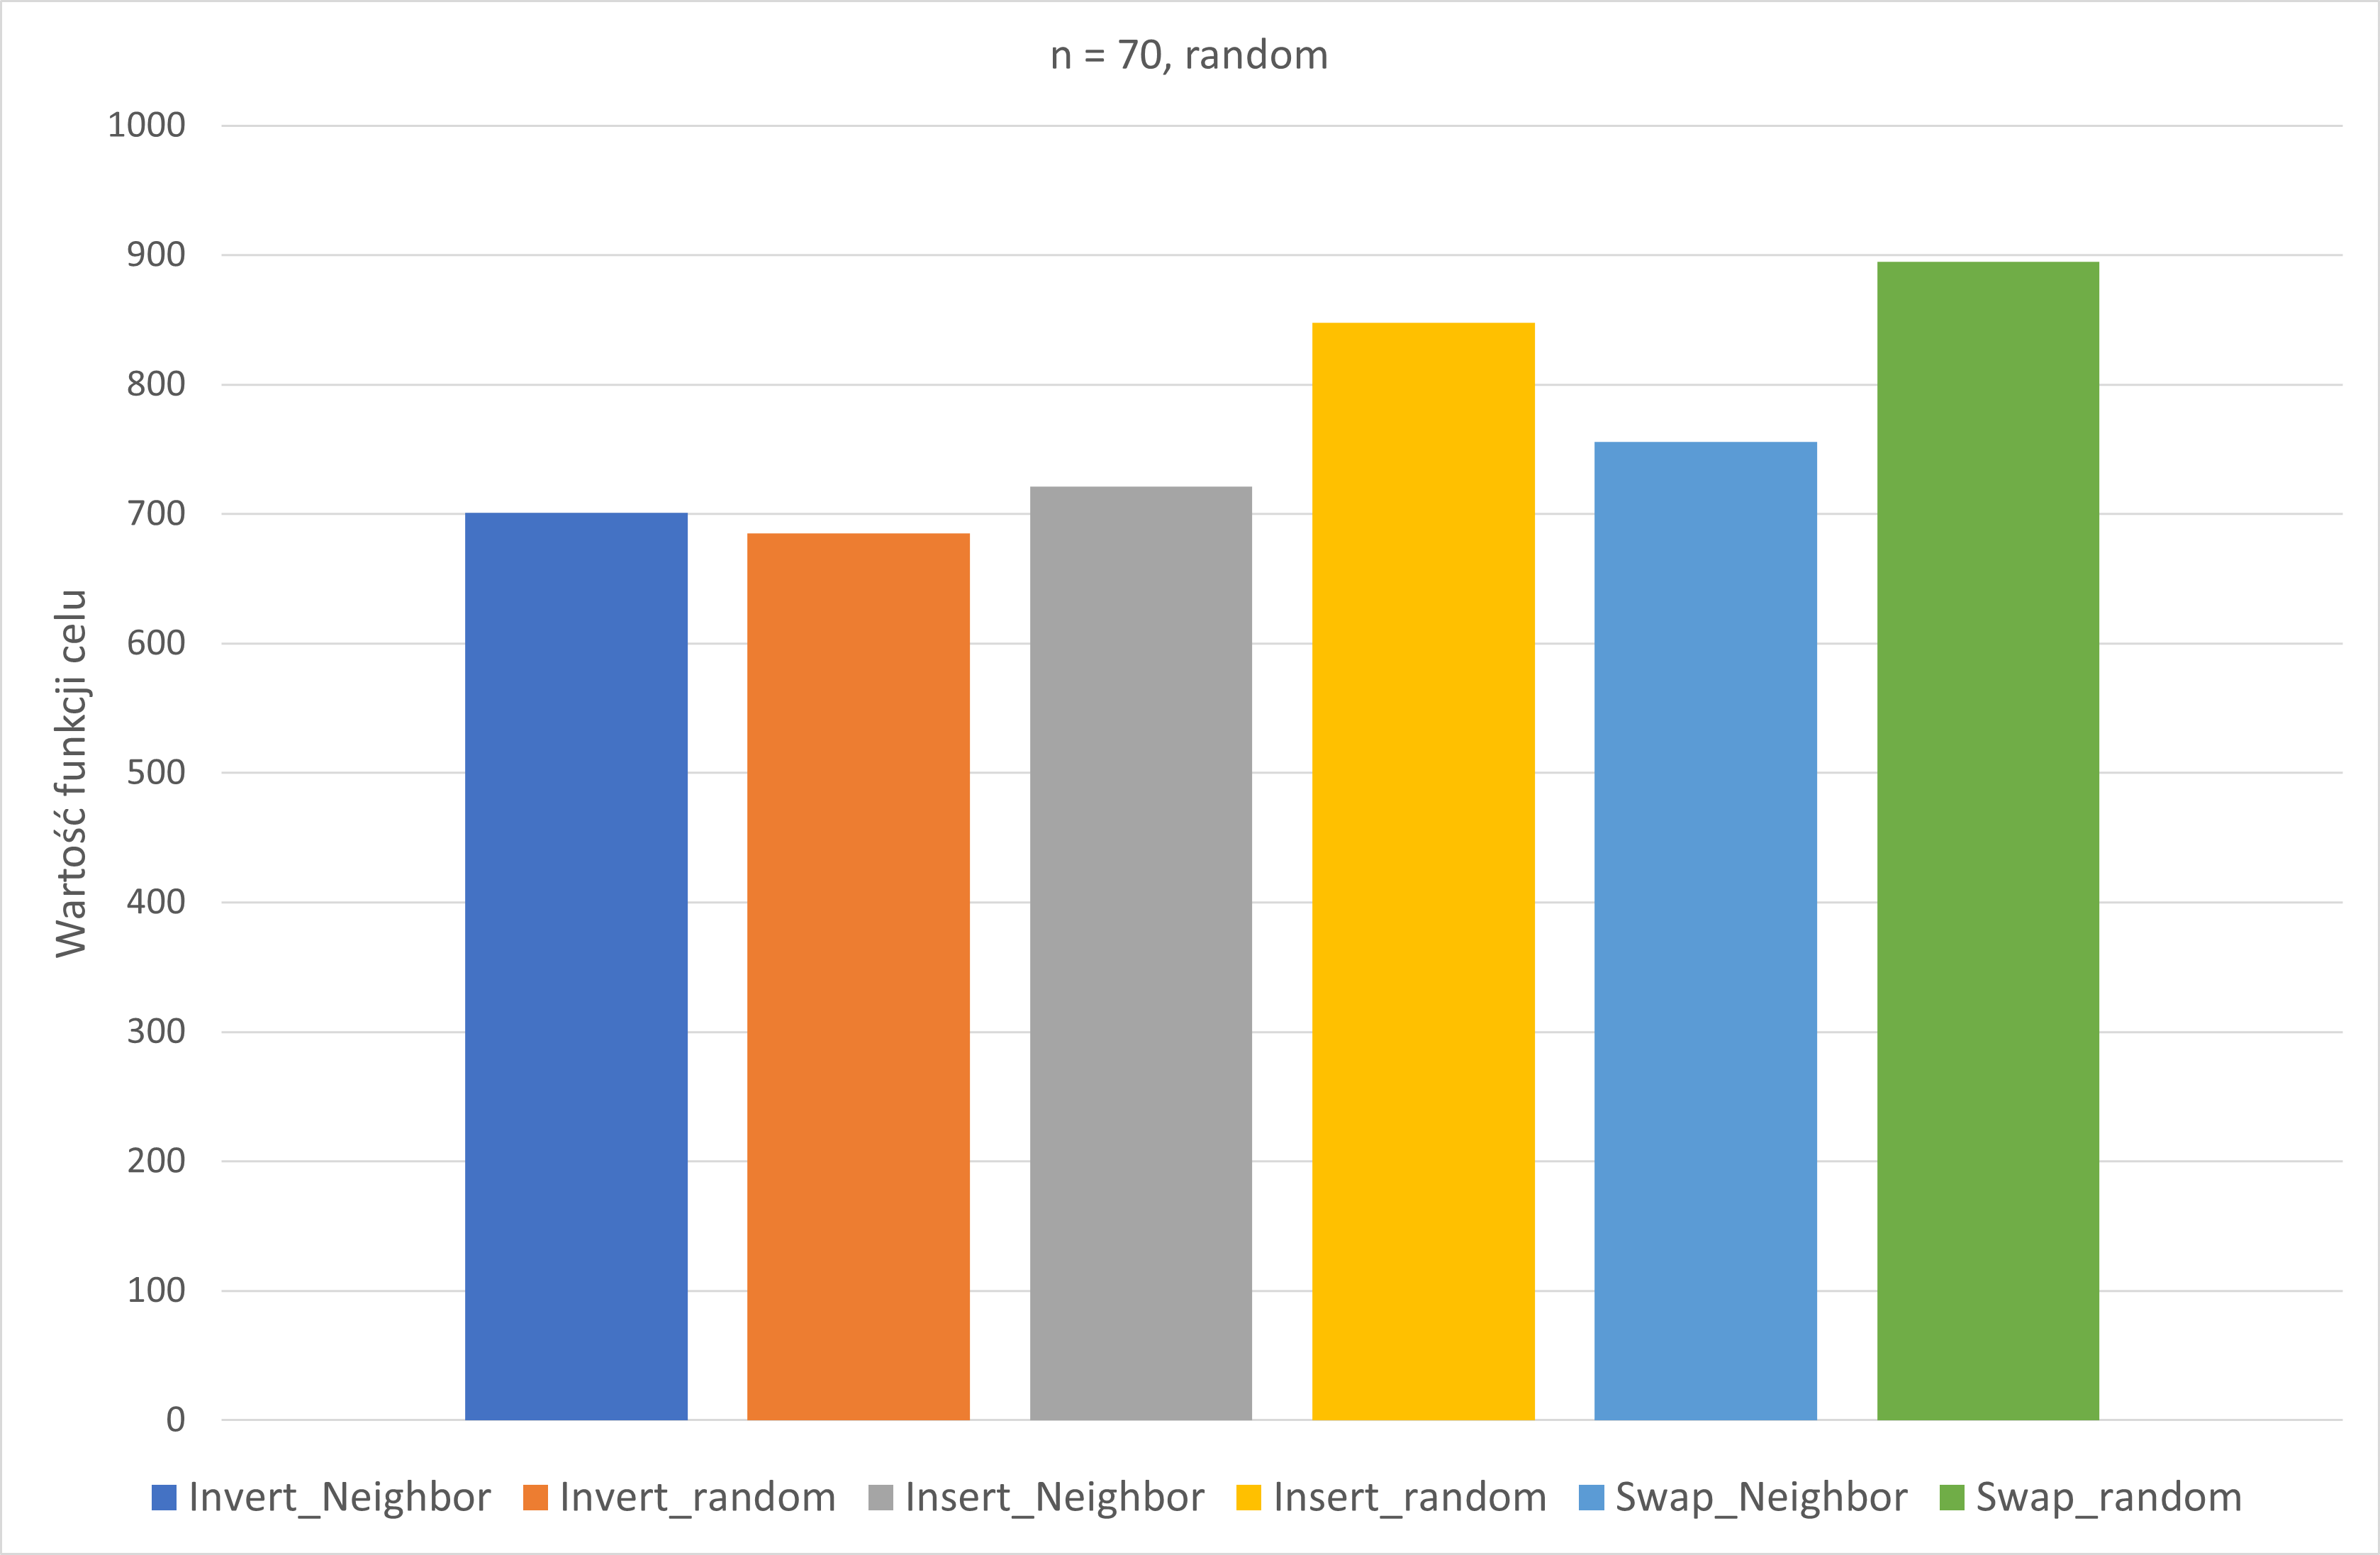
\includegraphics[scale=0.36]{70_rand}
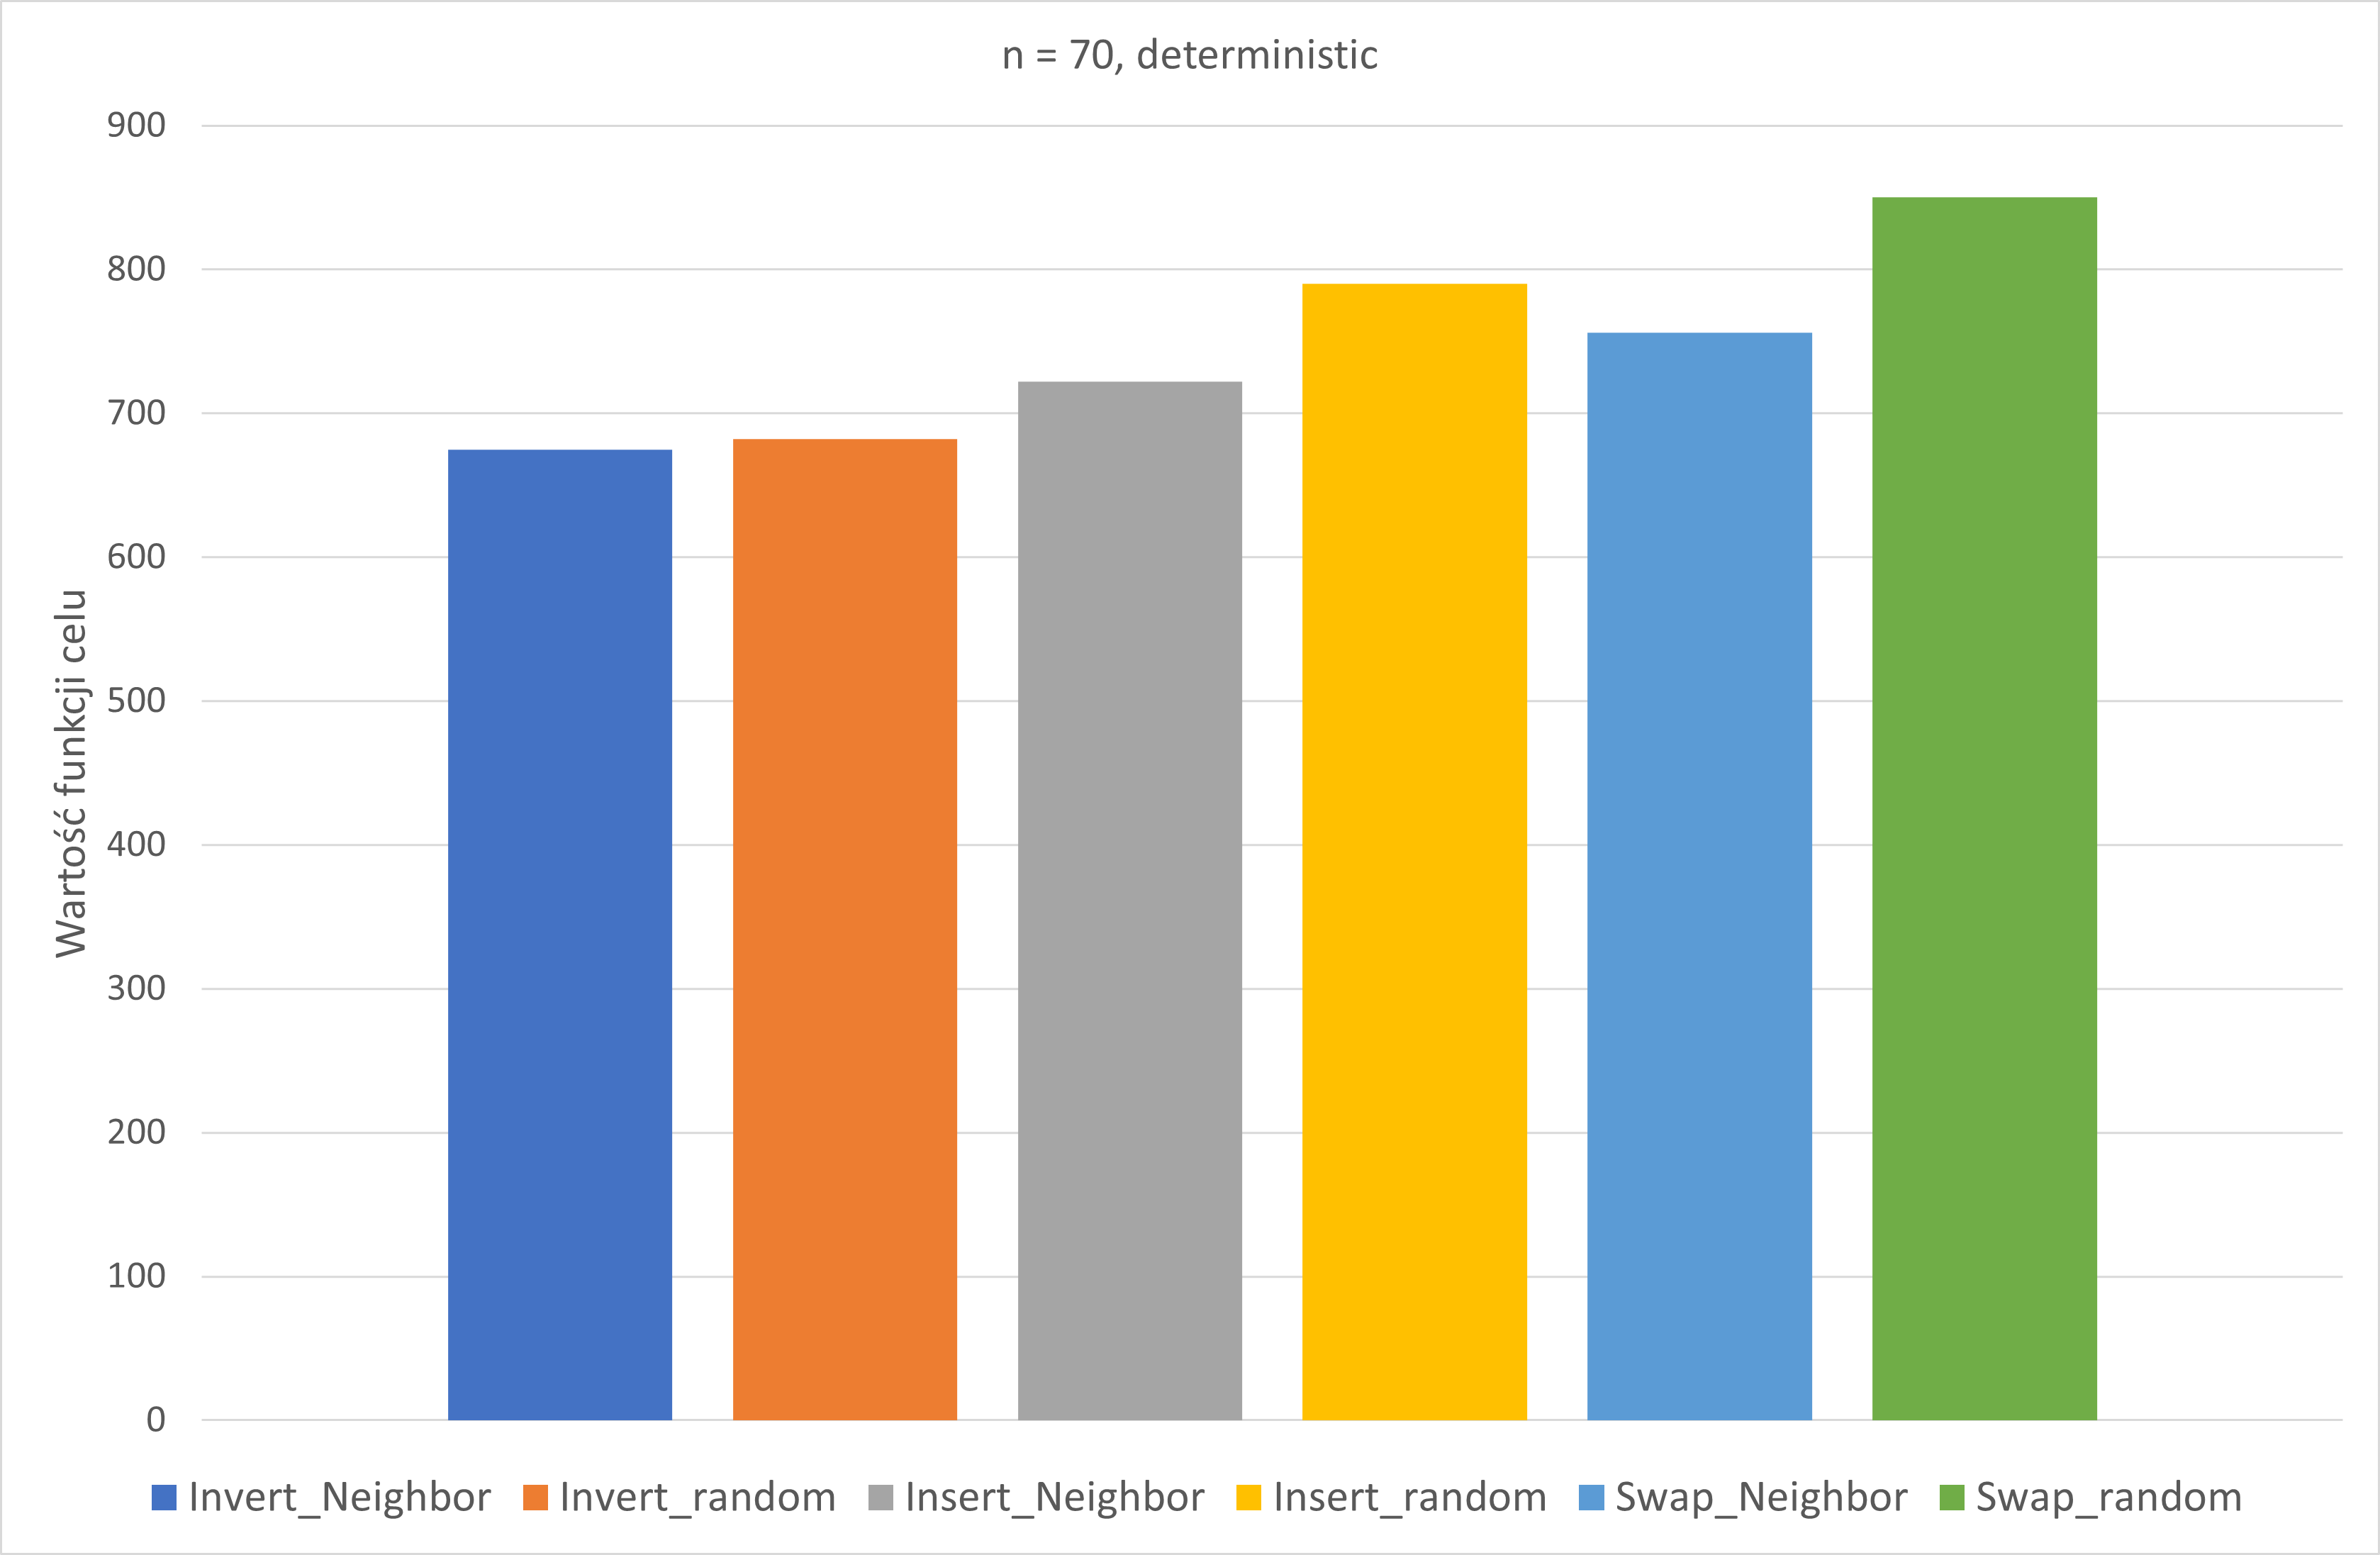
\includegraphics[scale=0.36]{70_deter}
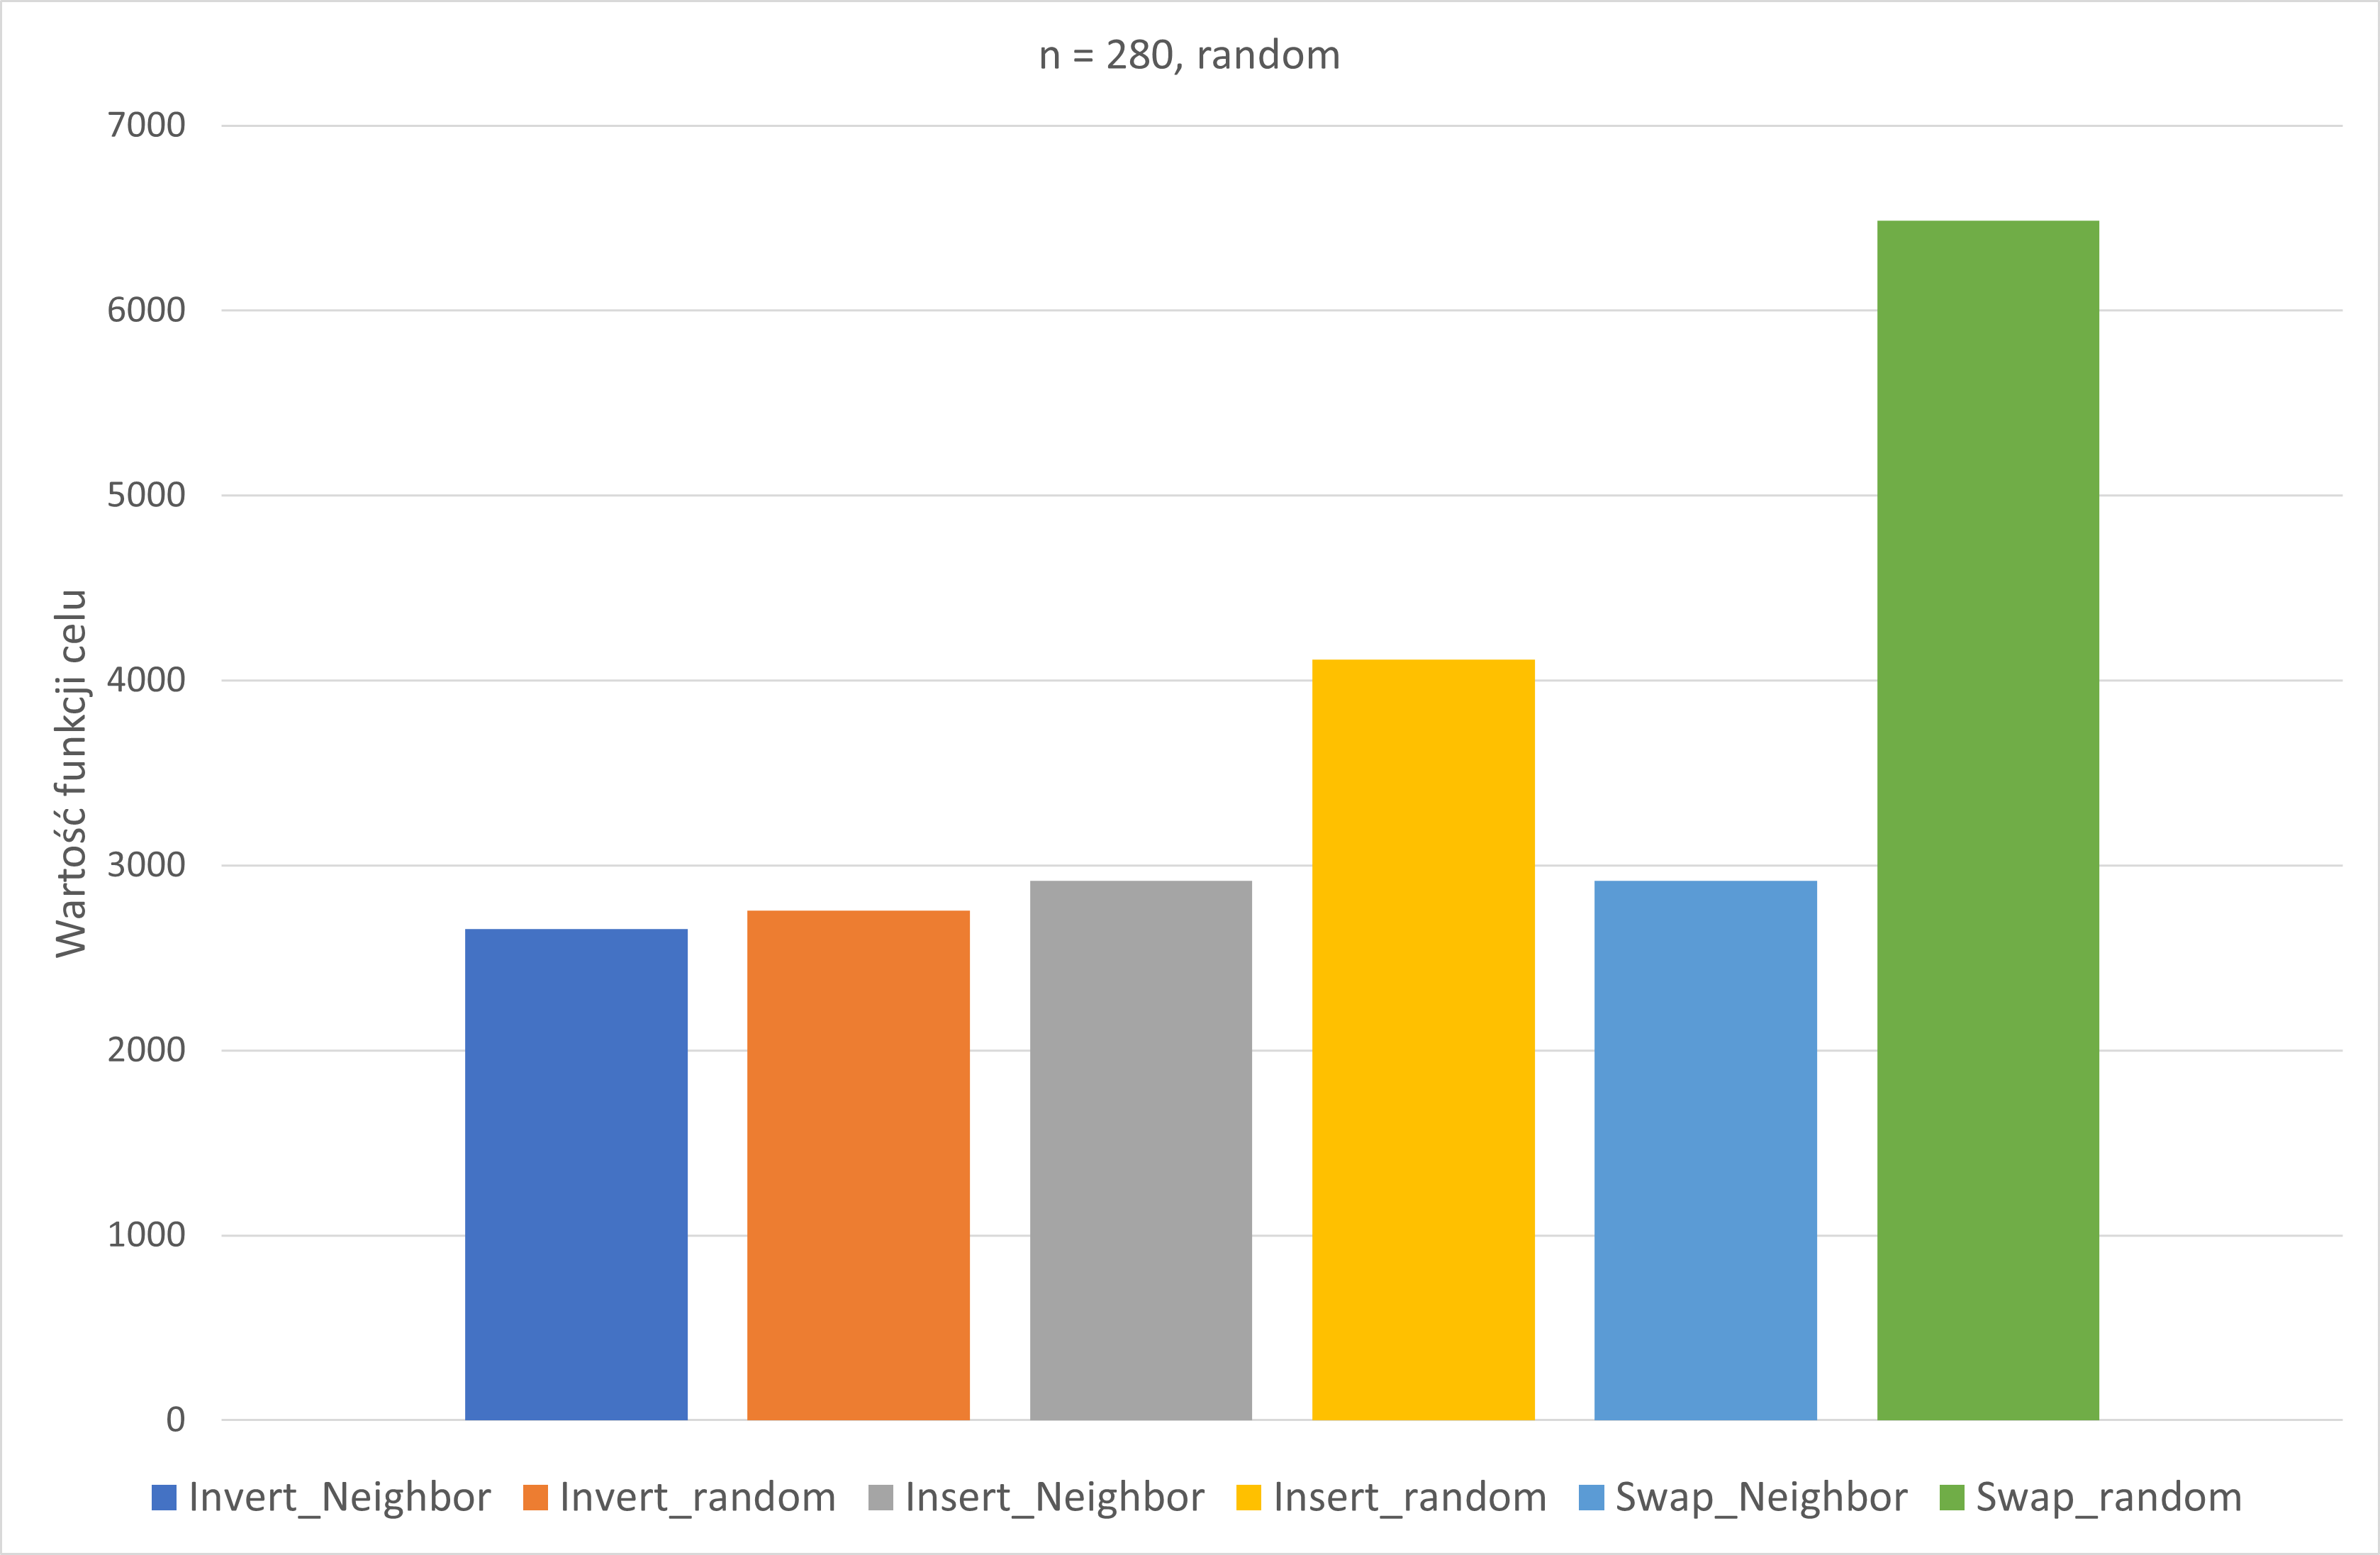
\includegraphics[scale=0.36]{280_rand}
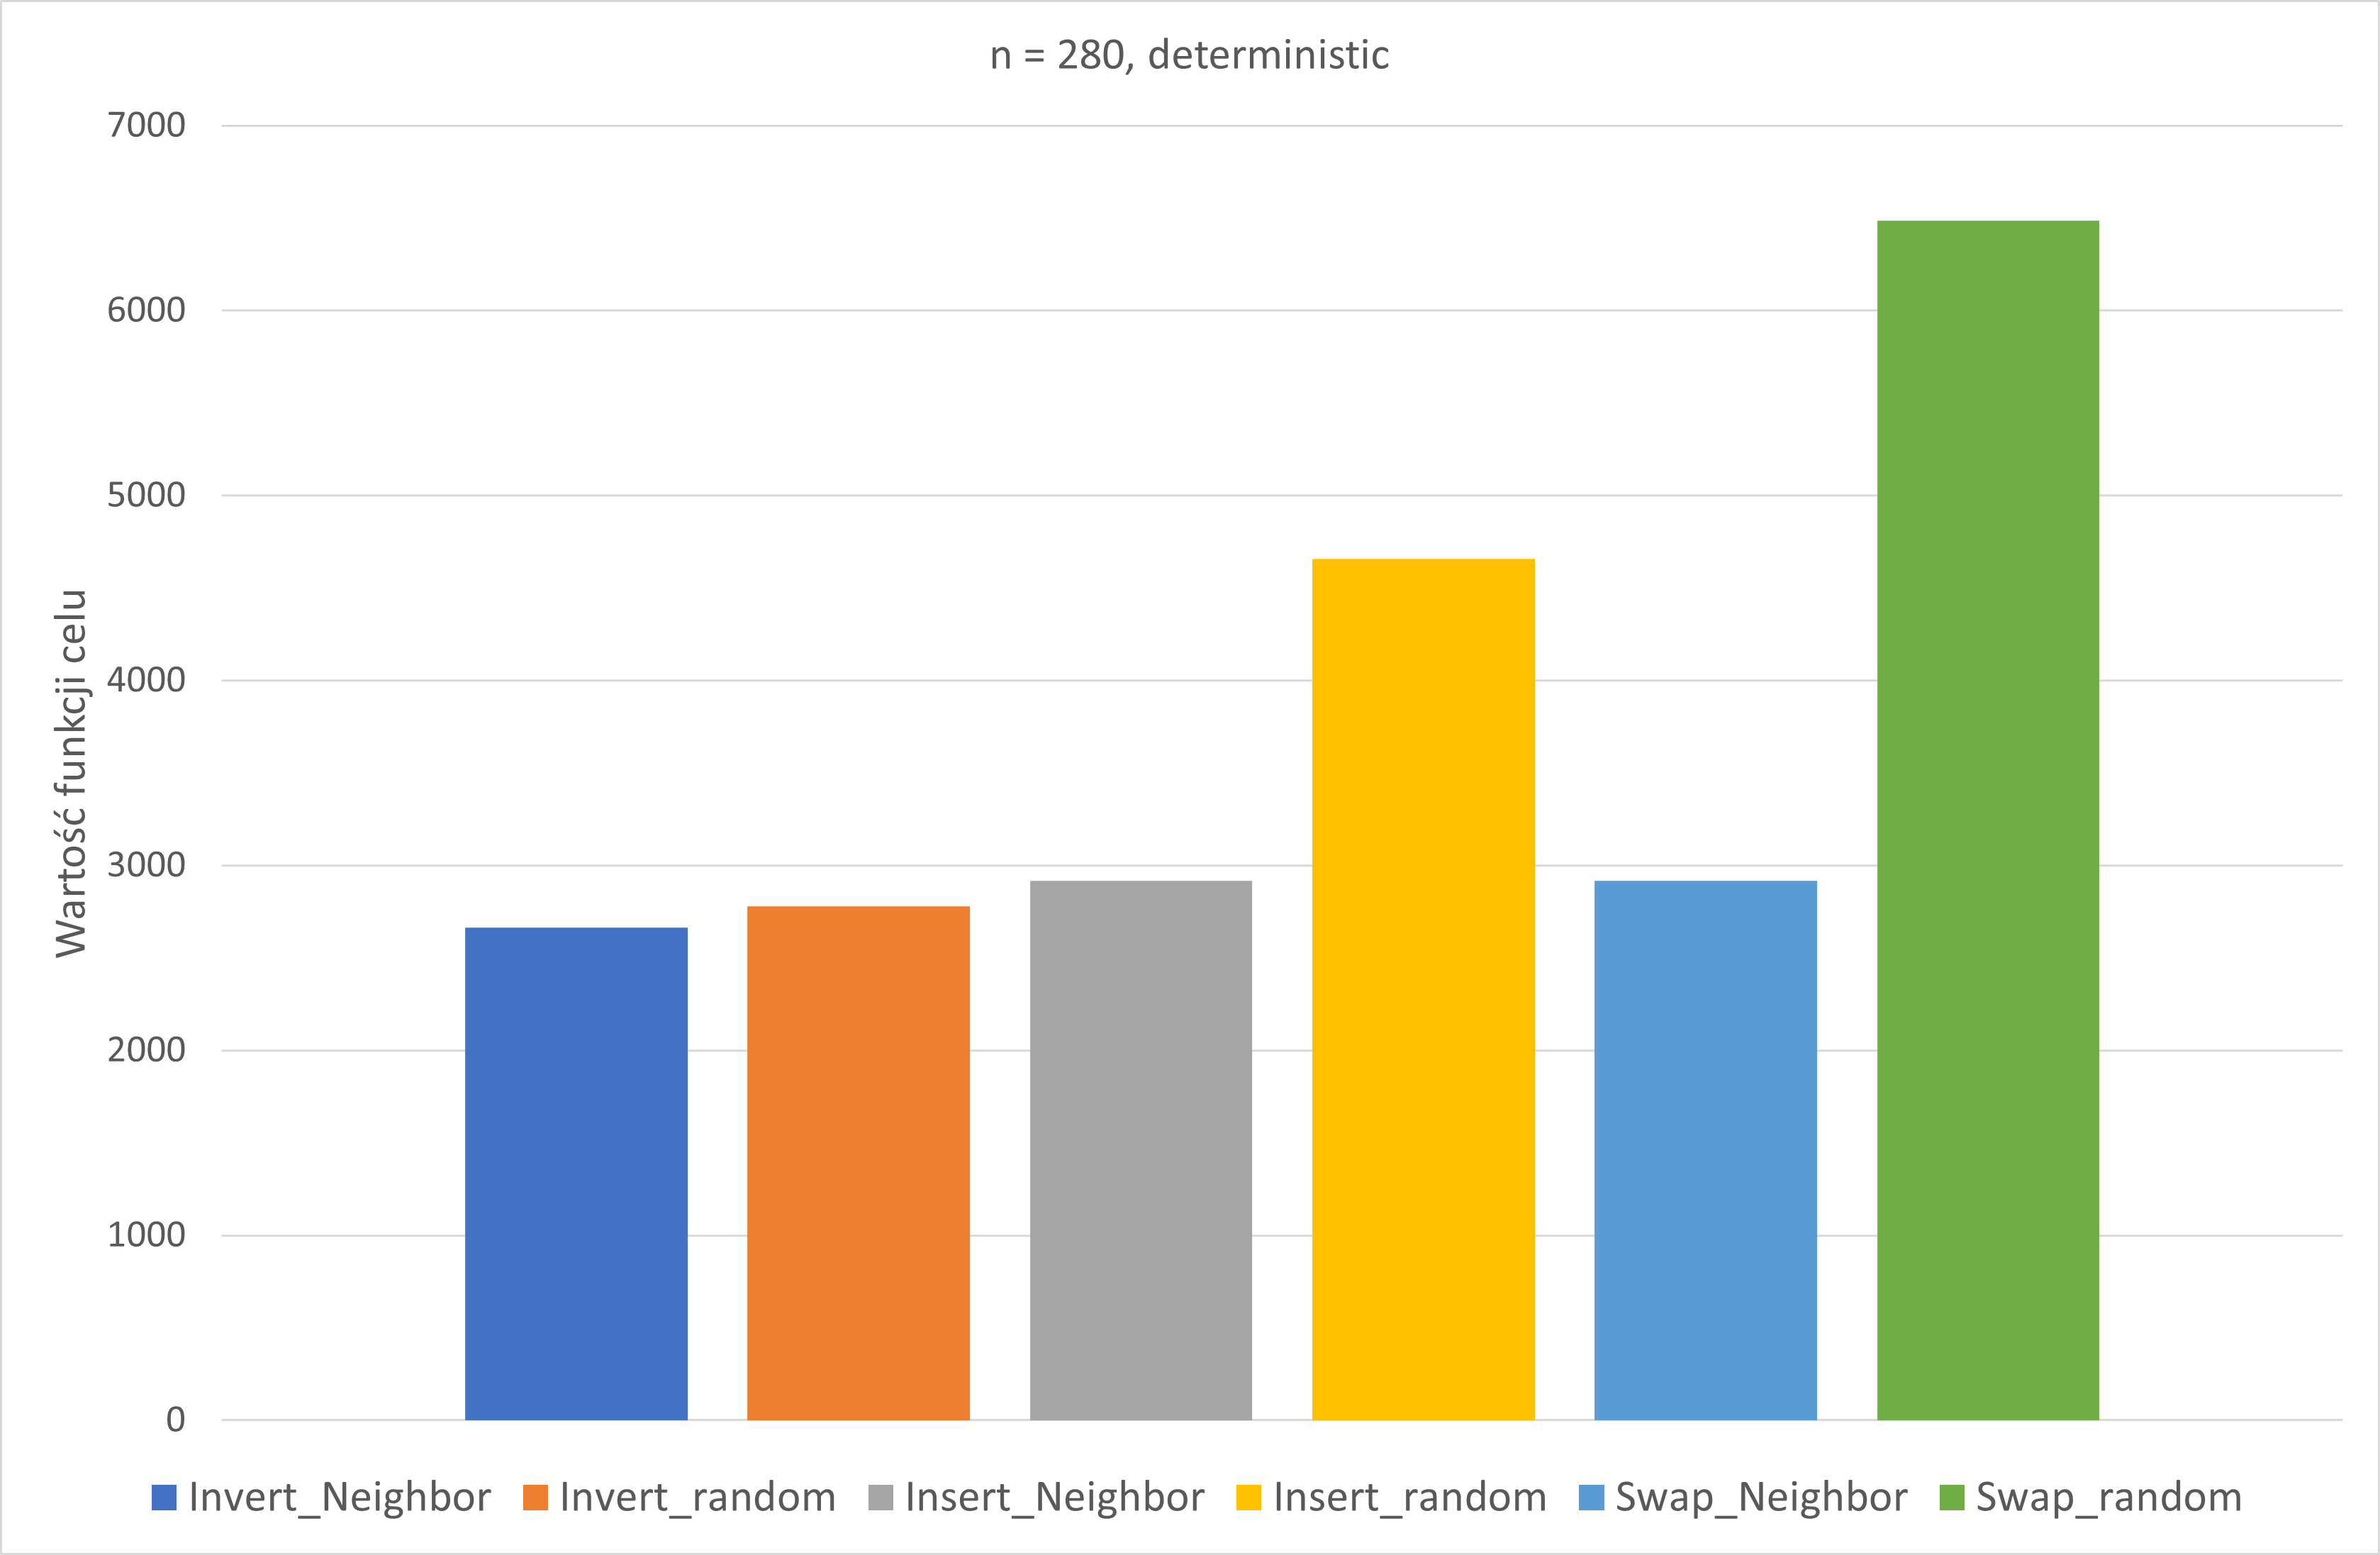
\includegraphics[scale=0.36]{280_deter}
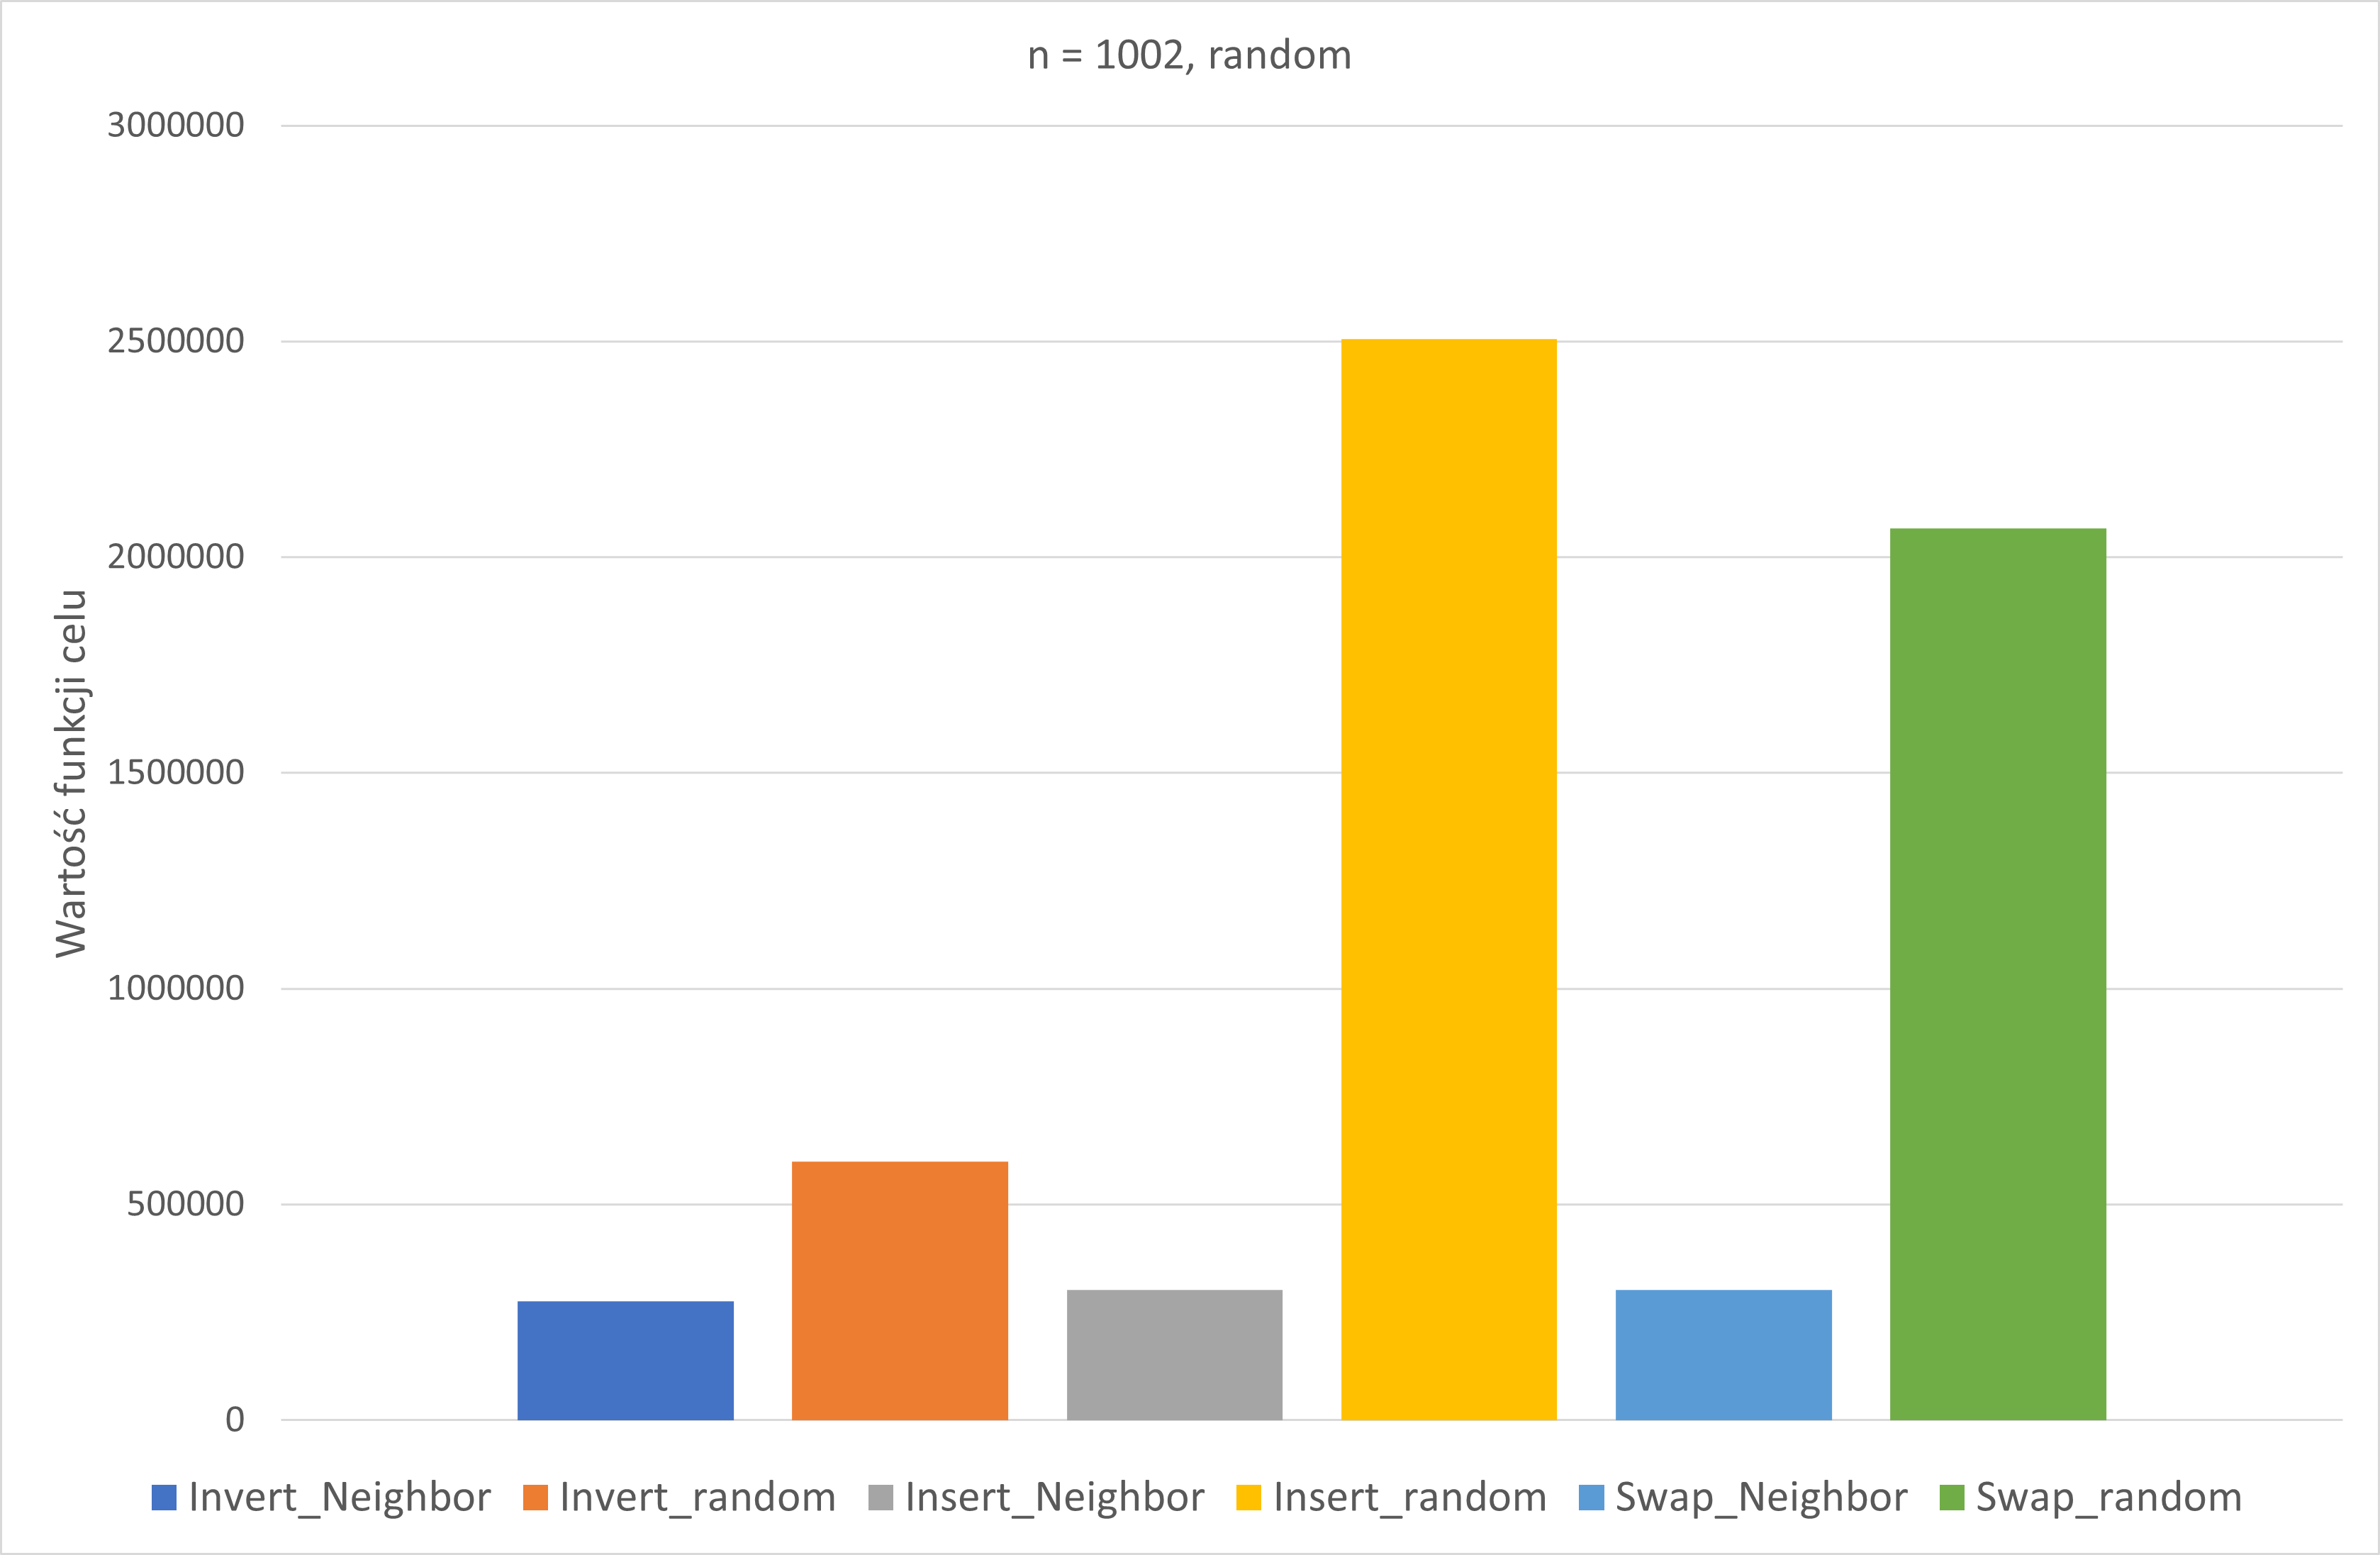
\includegraphics[scale=0.36]{1002_rand}
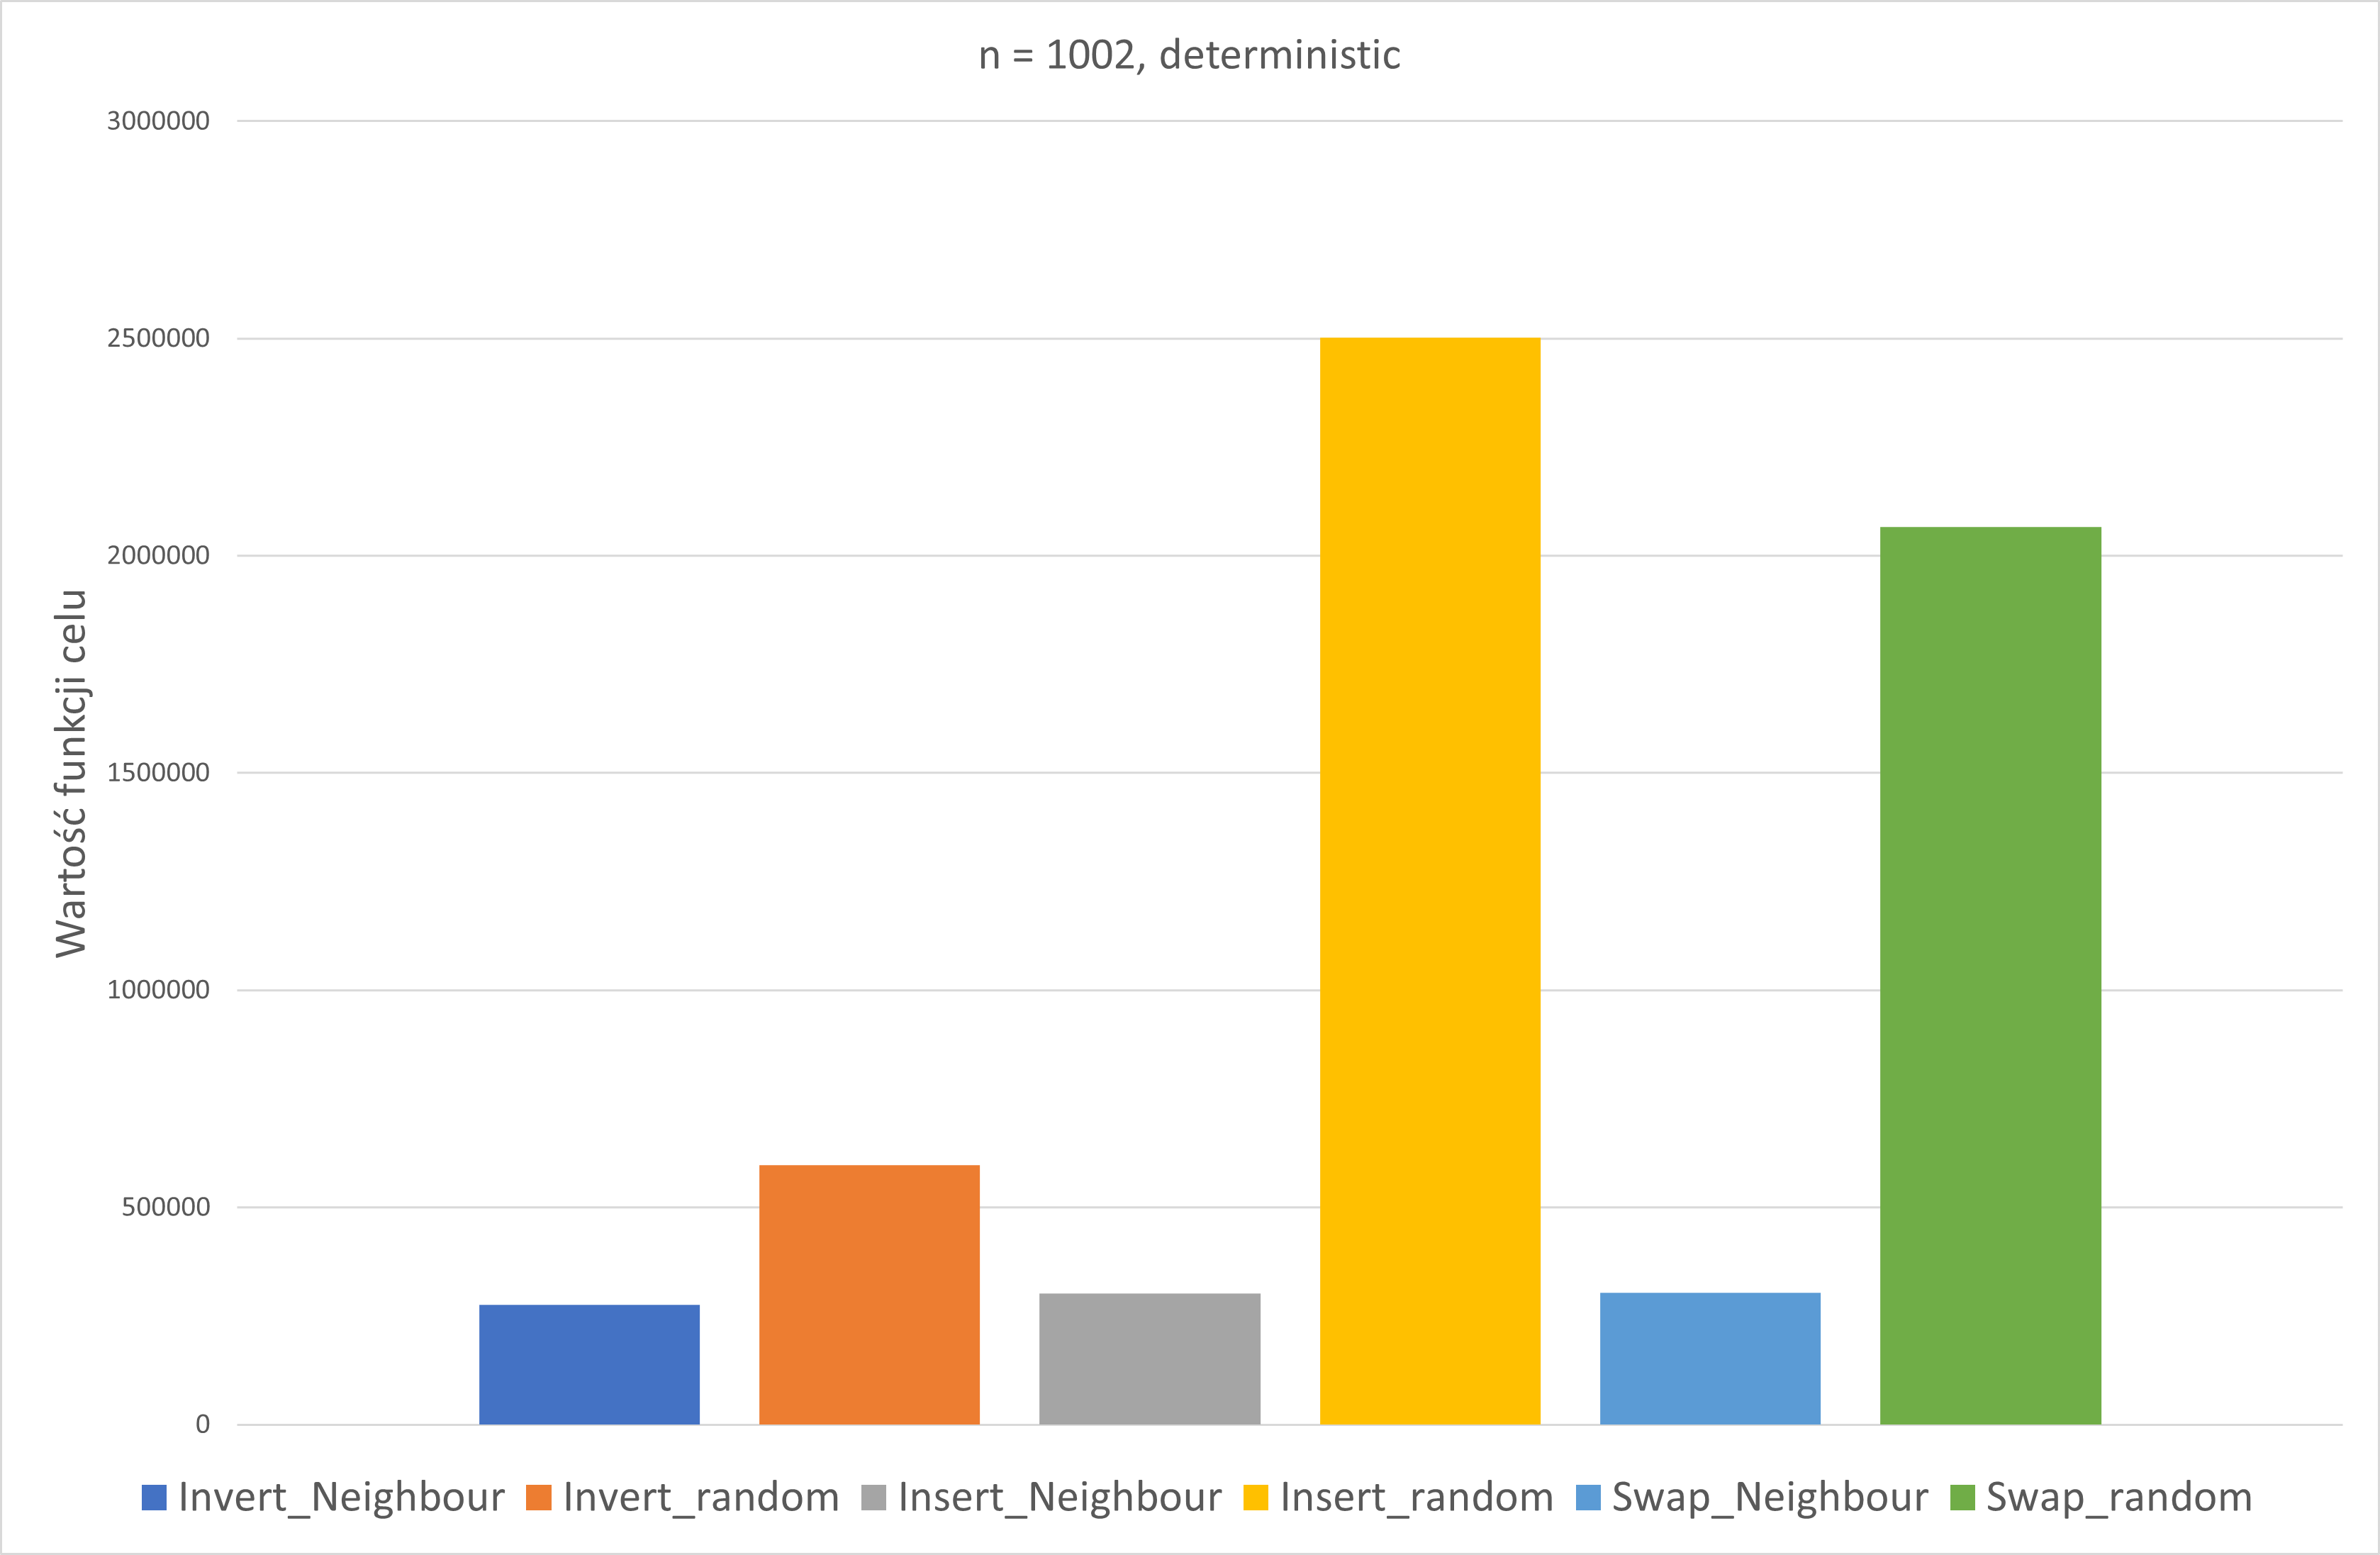
\includegraphics[scale=0.36]{1002_deter}

W obydwu wariantach operacji \texttt{kick} można zauważyć zbliżone wyniki przy wszystkich wielkościach problemu. Co więcej, wraz ze zwiększaniem się problemu bardziej klarownie widać różnice między wersjami. 
\begin{itemize}
	\item Początkowa trasa na podstawie Nearest Neighbour daje lepsze wyniki niż k-random
	\item Wszystkie otoczenia są porównywalne, najlepszy Invert, następnie Insert, najgorszy Swap
\end{itemize}


\subsubsection{Algorytmy uwspółbieżnione}

Uwspółbieżnienie zaimplementowano na zasadzie równoległego uruchamiania kilku instancji algorytmu \texttt{TABU-Search} jednocześnie. Z oczywistych względów nie testowano zachowania deterministycznej wersji algorytmu. Niestety, ta metoda uwspółbieżnienia nie dała dobrych rezultatów:

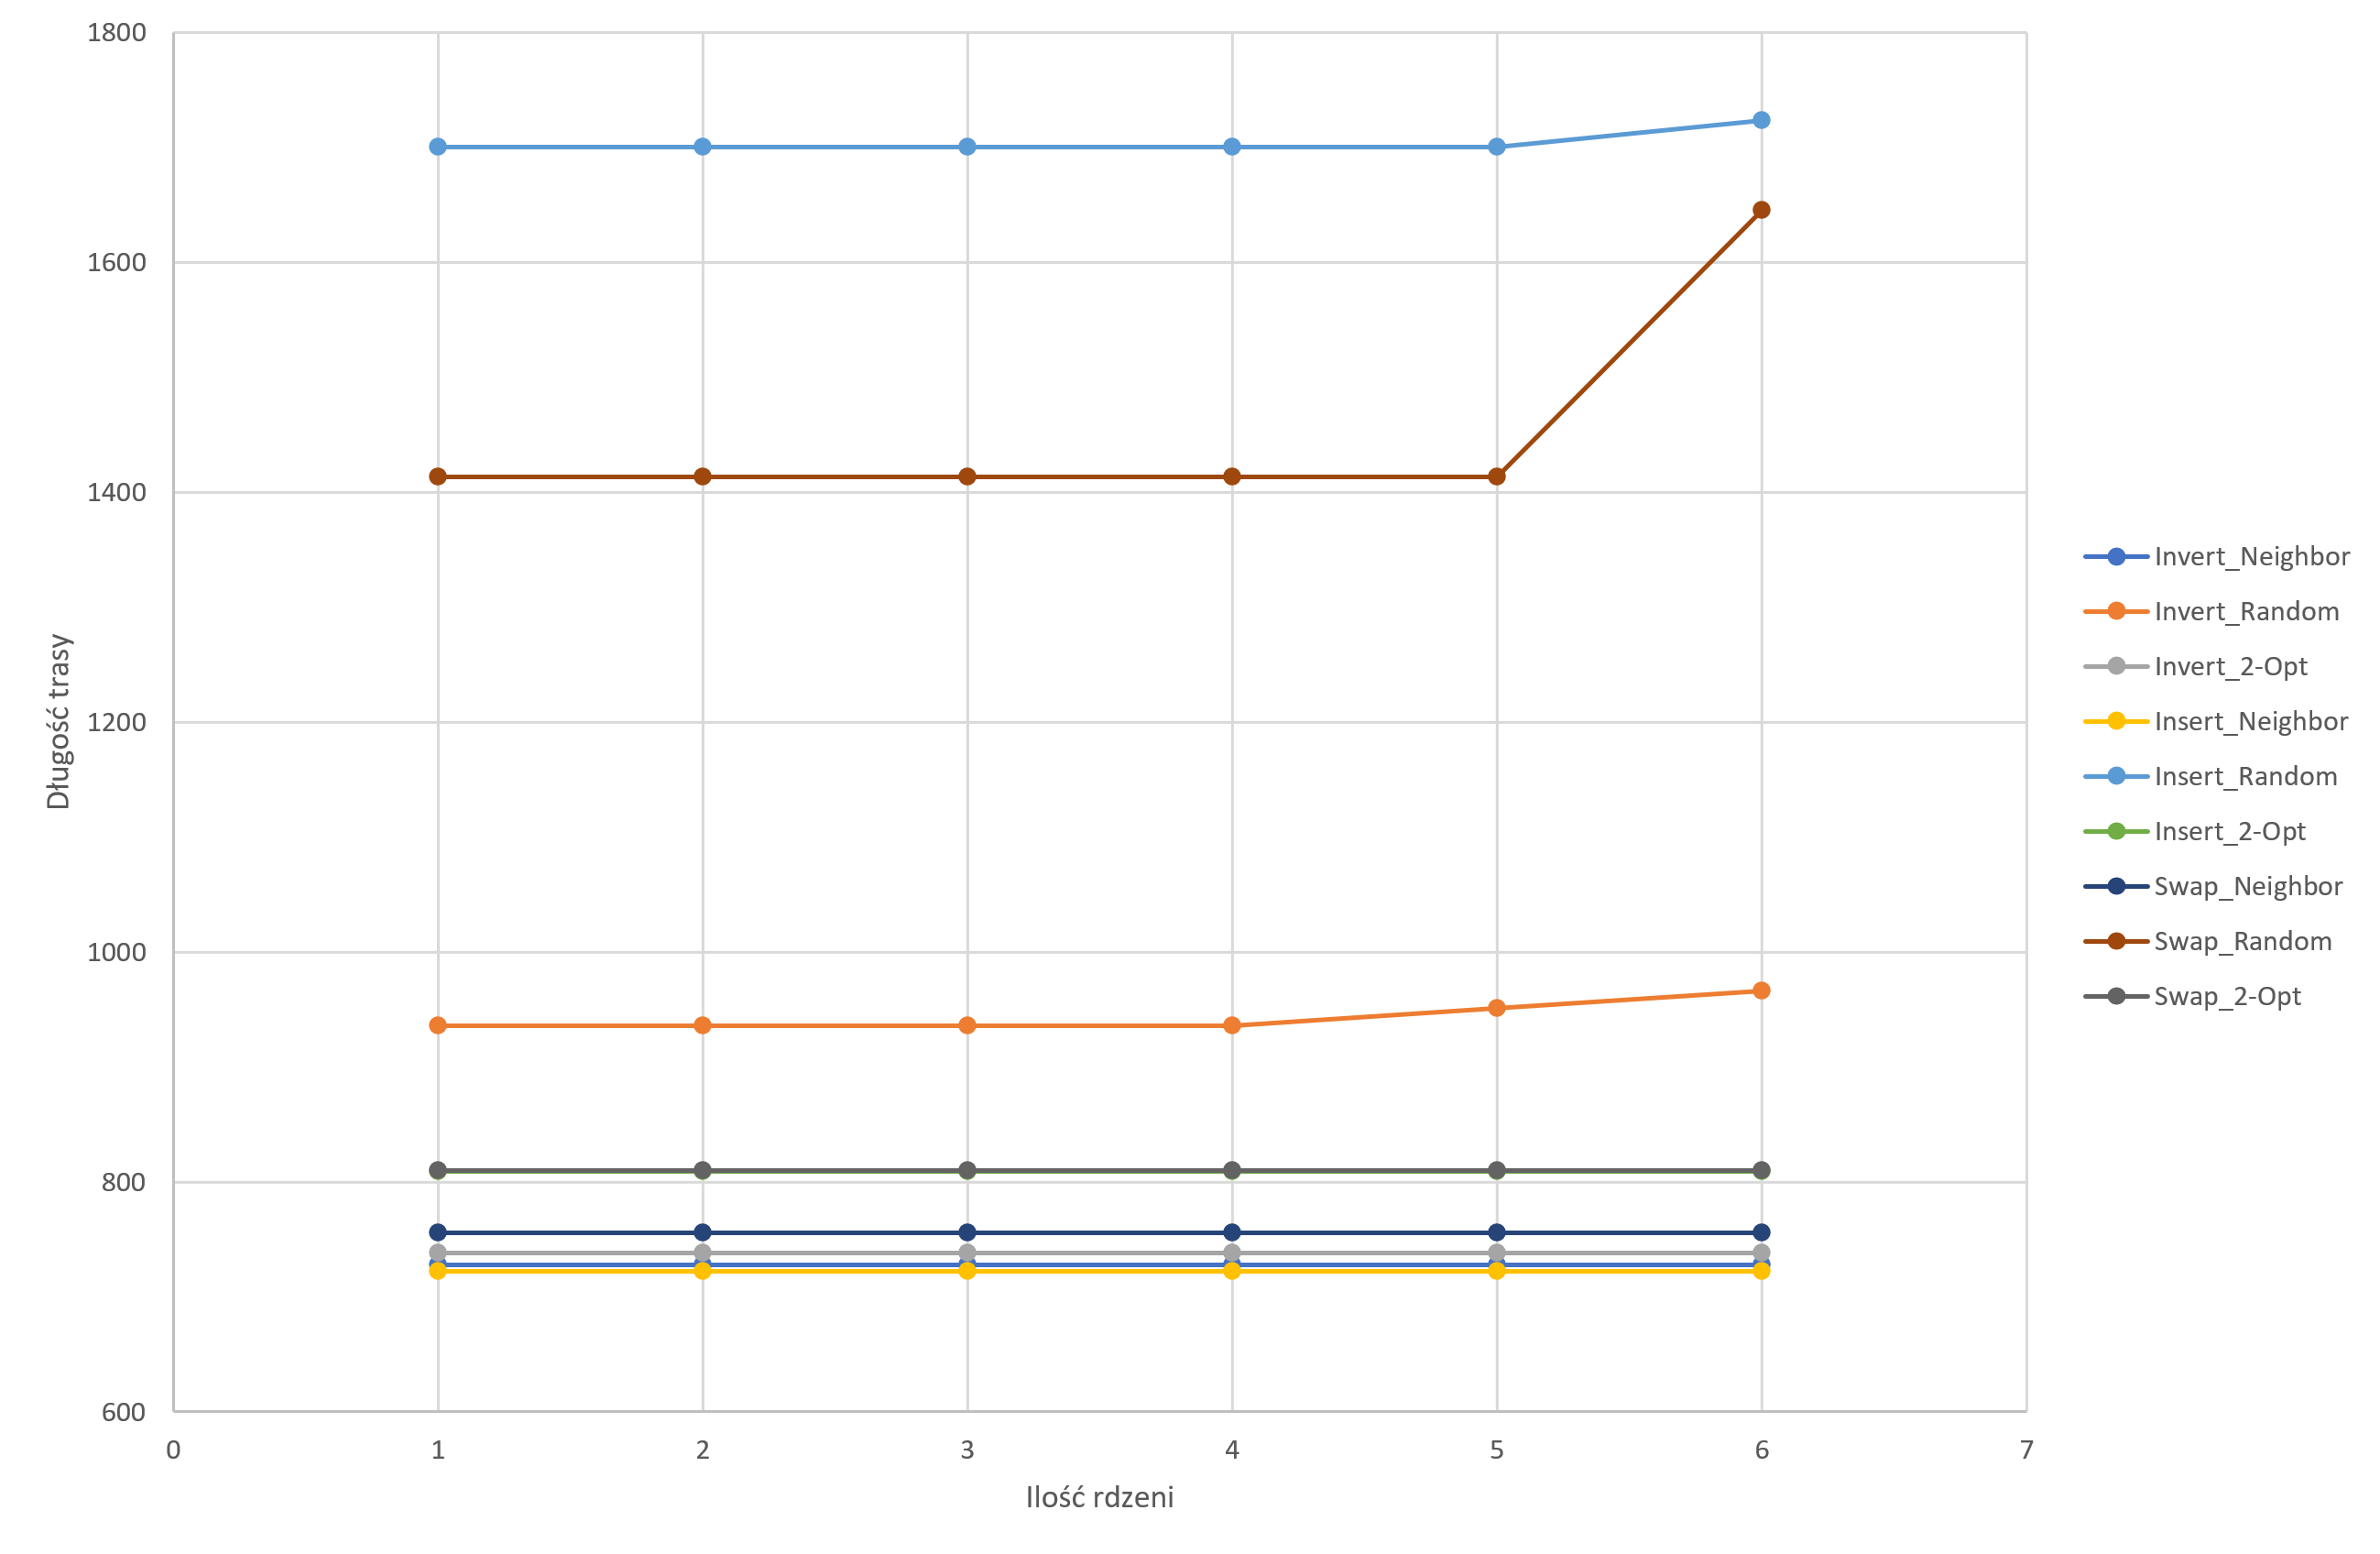
\includegraphics[scale=0.4]{parallel_n=70}

Dla każdego otoczenia i każdego rodzaju trasy startowej nie uzyskano w ten sposób polepszenia trasy.



\subsection{Wnioski}


\section*{Drobne uwagi}

\end{document}